\section{Market research}
\label{sec:market-research}
A TV remote is a device which is used to operate a television from
distance in a wireless mode. It also makes the TV usage simpler, more user friendly with its suggestive buttons. These buttons control functions such as power, volume, channel switch and various other features.

TV remotes are composed by the TV remote Shell,
the TV remote membrane, one LED and a data acquisition \& Infrared emitter PCB,
as illustrated in Fig.~\ref{fig:remotemat}. The unit cost of universal TV remotes is about 3 to 5 EUR.
%
% Remote material (side by side)
\begin{figure}[htb!]
  \centering
  %
  \begin{subfigure}{.4\textwidth}
  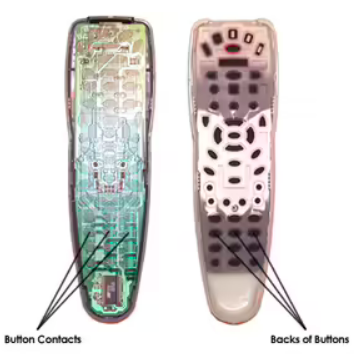
\includegraphics[width=\textwidth]{img/remotematerial1.png}%
  %\caption{KUKA's original position}%
  %\label{fig:ptp-test-orig}
\end{subfigure}
%
  \begin{subfigure}{.4\textwidth}
    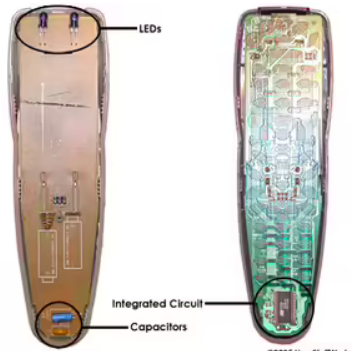
\includegraphics[width=\textwidth]{img/remotematerial2.png}%
%  \caption{KUKA's final position}%
%  \label{fig:ptp-test-final}
\end{subfigure}
%
  \caption{TV Remote control bill of materials, withdrawn from~\cite{remotematerial}}%
  \label{fig:remotemat}
\end{figure}

As can be seen in Fig.~\ref{fig:tvsells}, the amount of televisions sold per
year is about 200 million per year, with a tendency to increase over the next
years. Thus, at least the same amount of TV remotes sells is expected, as each
new TV requires one remote control, but it is expected to be exceeded due to TV
remote replacement arising from its malfunctioning or bad usage.
%
\begin{figure}[htb!]
\centering
    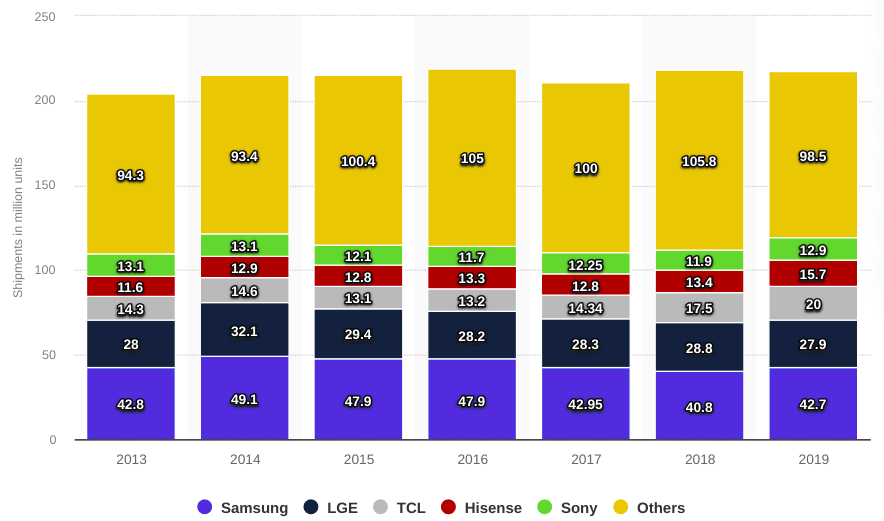
\includegraphics[width=0.7\columnwidth]{./img/tvsellings.png}
  \caption{Global LCD TV unit shipments from 2015 to 2019, by vendor (in
    millions), withdrawn from~\cite{tvsellings}}%
\label{fig:tvsells}
\end{figure}
%%% Local Variables:
%%% mode: latex
%%% TeX-master: "../../../dissertation"
%%% End:
